\documentclass[a4paper,12pt]{article}
\usepackage{enumitem}
\usepackage[utf8]{inputenc}
\usepackage[spanish]{babel}
\usepackage{amsmath,amsfonts,amssymb}
\usepackage[margin=0in, top=0.5in, bottom=0.5in, left=0.5in, right=0.5in]{geometry} % Márgenes sin superior
\usepackage{titlesec}
\usepackage{indentfirst}
\usepackage{listings} % Paquete para incluir código
\usepackage[usenames,dvipsnames]{color}
\usepackage{graphicx}
\usepackage{float}
\usepackage{csquotes}
\usepackage[table]{xcolor}% Para las filas a rayas
\usepackage{threeparttable} % Para notas debajo de la tabla
\usepackage{tabularx}
% \usepackage[backend=biber,style=numeric]{biblatex}
% \addbibresource{referencias.bib} % Archivo de bibliografía

\setlength{\parindent}{0pt}
\renewcommand{\lstlistingname}{Código}
\lstset{ 
  language=R,                     % the language of the code
  basicstyle=\ttfamily, % the size of the fonts that are used for the code
  numbers=left,                   % where to put the line-numbers
  numberstyle=\color{Blue},  % the style that is used for the line-numbers
  stepnumber=1,                   % the step between two line-numbers. If it is 1, each line
                                  % will be numbered
  numbersep=5pt,                  % how far the line-numbers are from the code
  backgroundcolor=\color{white},  % choose the background color. You must add \usepackage{color}
  showspaces=false,               % show spaces adding particular underscores
  showstringspaces=false,         % underline spaces within strings
  showtabs=false,                 % show tabs within strings adding particular underscores
  frame=single,                   % adds a frame around the code
  rulecolor=\color{black},        % if not set, the frame-color may be changed on line-breaks within not-black text (e.g. commens (green here))
  tabsize=2,                      % sets default tabsize to 2 spaces
  captionpos=b,                   % sets the caption-position to bottom
  breaklines=true,                % sets automatic line breaking
  breakatwhitespace=false,        % sets if automatic breaks should only happen at whitespace
  keywordstyle=\color{RoyalBlue},      % keyword style
  commentstyle=\color{YellowGreen},   % comment style
  extendedchars=true,
  literate={á}{{\'a}}1 {é}{{\'e}}1 {í}{{\'i}}1 {ó}{{\'o}}1 {ú}{{\'u}}1
} 
\titleformat{\section}
{\normalfont\fontsize{14.4}{18}\bfseries\raggedright}{}{0em}{}
\titleformat{\subsection}
{\normalfont\fontsize{12}{13}\bfseries\raggedright}{}{0em}{}

\begin{document}

% Portada personalizada
\begin{center}
  \centering

  {\LARGE \textbf{Universidad de Cuenca}}\\[0.2cm] % Título principal en negrita

  {\large Facultad de Ingeniería}\\[0.2cm] % Texto debajo del título principal
  {\large Maestría de Ciencia de Datos}\\[0.5cm] % Texto debajo del título principal

  {\Large \textbf{Aprendizaje Supervisado}}\\[0.2cm] % Texto relevante en negrita
  {\large Jaime P. Arevalo A., Esteban D. Vizhñay E.}\\[0.2cm]
  {\large \{paul.arevalo, esteban.vizhnay\}@ucuenca.edu.ec}\\[0cm]

  \rule{\linewidth}{0.30mm}\\[0.25cm] % Línea superior
  {\Large \textbf{Proyecto Final de Aprendizaje Supervisado}} % Título en negrita
  \rule{\linewidth}{0.30mm} % Línea inferior

\end{center}

\begin{abstract}
  Este estudio tiene como objetivo predecir el rendimiento académico de los estudiantes influido con el consumo del alcohol, medido en porcentaje de calificaciones, utilizando un modelo de regresión lineal basado en diversos factores relacionados con el rendimiento. Los factores considerados incluyen la relación con los padres, la mesada mensual, la facultad, el estado de la beca, las horas de estudio y la vida social del estudiante. Se recopiló un conjunto de datos de estudiantes, que eventualmente fue preprocesado para la normalización y la codificación de variables categóricas. Se construyó un modelo de regresión lineal para establecer relaciones entre estos factores y el rendimiento académico. La evaluación del modelo se realizó utilizando métricas como el Error Cuadrático Medio (MSE) y el coeficiente de determinación (R²). Los resultados indican que el modelo de regresión lineal puede ser determinante para predecir el rendimiento de los estudiantes, con ciertos factores teniendo un impacto más significativo en el rendimiento académico que otros. Estos hallazgos pueden informar estrategias para apoyar a los estudiantes y mejorar sus resultados académicos.
\end{abstract}

\section{Introducción}

\subsection{Problema a abordar}
El consumo excesivo de alcohol puede perjudicar a un estudiante universitario de diversas maneras ya sea a nivel académico, salud, mental, social entre otras. En general el consumo de alcohol es un problema grave que afecta a la mayoría de comunidad universitaria a nivel global, está claro que esta afecta negativamente a los estudiantes de diversas maneras pero es necesario obtener un panorama general de cómo afecta al rendimiento académico, esto puede permitir a realizar campañas de socialización, toma de decisiones informadas para mitigar o reducir esta problemática.
\subsection{Justificación de la importancia del problema}
El consumo de alcohol perjudica a las metas educativas de una institución a consecuencia de bajo rendimiento académico, pérdidas de año, inasistencia, daños a la propiedad, irrespeto a las normas de convivencia universitaria, robos, autolesiones, entre otros. Las encuestas a la comunidad universitaria permiten conocer un panorama más amplio del mismo para poder proponer soluciones ante las situaciones presentadas.
\subsection{Objetivos del trabajo}
Realizar un análisis estadístico descriptivo, análisis exploratorio de datos y realizar un modelo de clasificación que permita predecir el rendimiento escolar del entrevistado.

\section{Revisión de literatura}
La literatura existente sobre el consumo del alcohol y su relación con el rendimiento académico evidencia que mientras aumenta el número de noches destinadas a la ingesta de alcohol, el rendimiento de los estudiantes disminuye significativamente (Matt, Shannon, \& Oliver, 2012). De acuerdo al estudio realizado por (Singleton \& Wolfston, 2009) el consumo del alcohol, horas de sueño, tiempo de estudio y el rendimiento están estrechamente relacionadas, los estudiantes que consumen en exceso alcohol destinan menos horas de sueño y tiempo de estudio que provoca patrones de sueño deficientes afectando negativamente su rendimiento académico. Por otra parte (Idoko, Muyiwa, \& Agoha, 2015) entrevistaron a 200 estudiantes universitarios donde su objetivo era probar tres hipótesis: i) Relación positiva entre el alcohol y rendimiento académico, ii) Diferencia significativa entre estudiantes consumidores y no consumidores en su rendimiento académico, iii) Efecto significativo entre el consumo de alcohol y el rendimiento académico. El estudio arrojó los siguientes resultados: i) 66\% estudiantes faltaban a clases o reprobaron un examen a causa de una resaca, ii) 39\% estudiantes fueron sancionados por consumo de alcohol por parte de la universidad.  El estudio concluyó que si existe una relación significativa entre el consumo y el rendimiento académico. De la misma manera (Madson, Zeigler-Hill, Noble \& Mohn , 2014) descubrió que muchos estudiantes con problemas de ansiedad social bebían para mejorar y ser aceptados por sus compañeros de clases y aumentar su estado de ánimo, los mismos creen que beber les ayudará a encajar con sus compañeros y el entorno que los rodea. A partir del aumento de la ingesta de alcohol existieron consecuencias negativas en los estudiantes en diferentes ámbitos: personal, académico, salud y mental. La idea anterior es apoyada por (White, 2013) que describe que el consumo de alcohol en los estudiantes universitarios provoca bajo rendimiento académico, abuso del mismo, dependencias, muertes, pérdidas de memoria y cambios en la función cerebral.

\section{Descripción de la fuente de datos}
El conjunto de datos utilizado proviene de un estudio realizado en la Universidad de Stellenbosch. Este realizó una encuesta a 406 estudiantes de diferentes años académicos abordando diferentes aspectos del mismo como  rendimiento escolar, promedio anterior, horas adicionales de estudio, entre otros.

\begin{table}[H]
  \centering
  \resizebox{\textwidth}{!}{ % Ajusta automáticamente la tabla al ancho de la página
    \begin{threeparttable}
      \begin{tabularx}{\textwidth}{|p{0.35\textwidth}|p{0.35\textwidth}|p{0.125\textwidth}|X|}
        \hline
        \rowcolor{gray!20} % Fila rayada
        Variable                                                                                         & Descripción                                                                         & Tipo         & Tipo de Dato \\
        \hline
        Your Sex?                                                                                        & Sexo del estudiante                                                                 & Cualitativa  & Cadena       \\
        \rowcolor{gray!10} % Fila rayada
        Your Matric (grade 12) Average/GPA (in \%)                                                       & Rendimiento escolar en porcentaje                                                   & Cuantitativa & Decimal      \\
        What year were you in last year (2023)?                                                          & Año en el que estaba el estudiante en 2023                                          & Cualitativa  & Cadena       \\
        \rowcolor{gray!10} % Fila rayada
        What faculty does your degree fall under?                                                        & Facultad a la que pertenece el grado del estudiante                                 & Cualitativa  & Cadena       \\
        Your 2023 academic year average/GPA in \% (Ignore if you are 2024 1st year student)              & Promedio académico del año 2023 en porcentaje                                       & Cuantitativa & Decimal      \\
        \rowcolor{gray!10} % Fila rayada
        Your Accommodation Status Last Year (2023)                                                       & Estado de alojamiento del estudiante en 2023                                        & Cualitativa  & Cadena       \\
        Monthly Allowance in 2023                                                                        & Mesada mensual en 2023                                                              & Cuantitativa & Decimal      \\
        \rowcolor{gray!10} % Fila rayada
        Were you on scholarship/bursary in 2023?                                                         & Beca o financiamiento en 2023                                                       & Cualitativa  & Cadena       \\
        Additional amount of studying (in hrs) per week                                                  & Horas adicionales de estudio por semana                                             & Cuantitativa & Decimal      \\
        \rowcolor{gray!10} % Fila rayada
        How often do you go out partying/socialising during the week?                                    & Frecuencia de salidas sociales durante la semana                                    & Cualitativa  & Cadena       \\
        On a night out, how many alcoholic drinks do you consume?                                        & Número de bebidas alcohólicas consumidas en una salida nocturna                     & Cuantitativa & Decimal      \\
        \rowcolor{gray!10} % Fila rayada
        How many classes do you miss per week due to alcohol reasons (i.e: being hungover or too tired)? & Clases perdidas por razones relacionadas con el alcohol                             & Cualitativa  & Cadena       \\
        How many modules have you failed thus far into your studies?                                     & Cantidad de módulos que el estudiante ha reprobado hasta el momento en sus estudios & Cuantitativa & Decimal      \\
        \rowcolor{gray!10} % Fila rayada
        Are you currently in a romantic relationship?                                                    & ¿El estudiante actualmente está en una relación romántica?                          & Cualitativa  & Cadena       \\
        Do your parents approve alcohol consumption?                                                     & Aprobación del consumo de alcohol por parte de los padres                           & Cualitativa  & Cadena       \\
        \rowcolor{gray!10} % Fila rayada
        How strong is your relationship with your parent/s?                                              & Relación con los padres                                                             & Cualitativa  & Cadena       \\
        \hline
      \end{tabularx}
    \end{threeparttable}
  } % Cierre de \resizebox
  \caption{Descripión de las variables}
\end{table}

\section{Metodología}
\subsection{Técnicas de análisis de datos utilizadas}

\begin{itemize}[label=\textbullet] % Cambia el tipo de viñeta
  \item Preparación de los datos: formatos, datos ausentes, columnas nuevas.
        \begin{itemize}
          \item Estadística descriptiva.
          \item Gráficas.
        \end{itemize}
  \item Pruebas estadísticas para el análisis bivariable y multivariable
        \begin{itemize}
          \item Regresion lineales
          \item SVR
          \item Arboles de Decisión
          \item Random Forest
        \end{itemize}
\end{itemize}

\subsection{Estadística descriptiva.}
\begin{figure}[H]
  \centering
  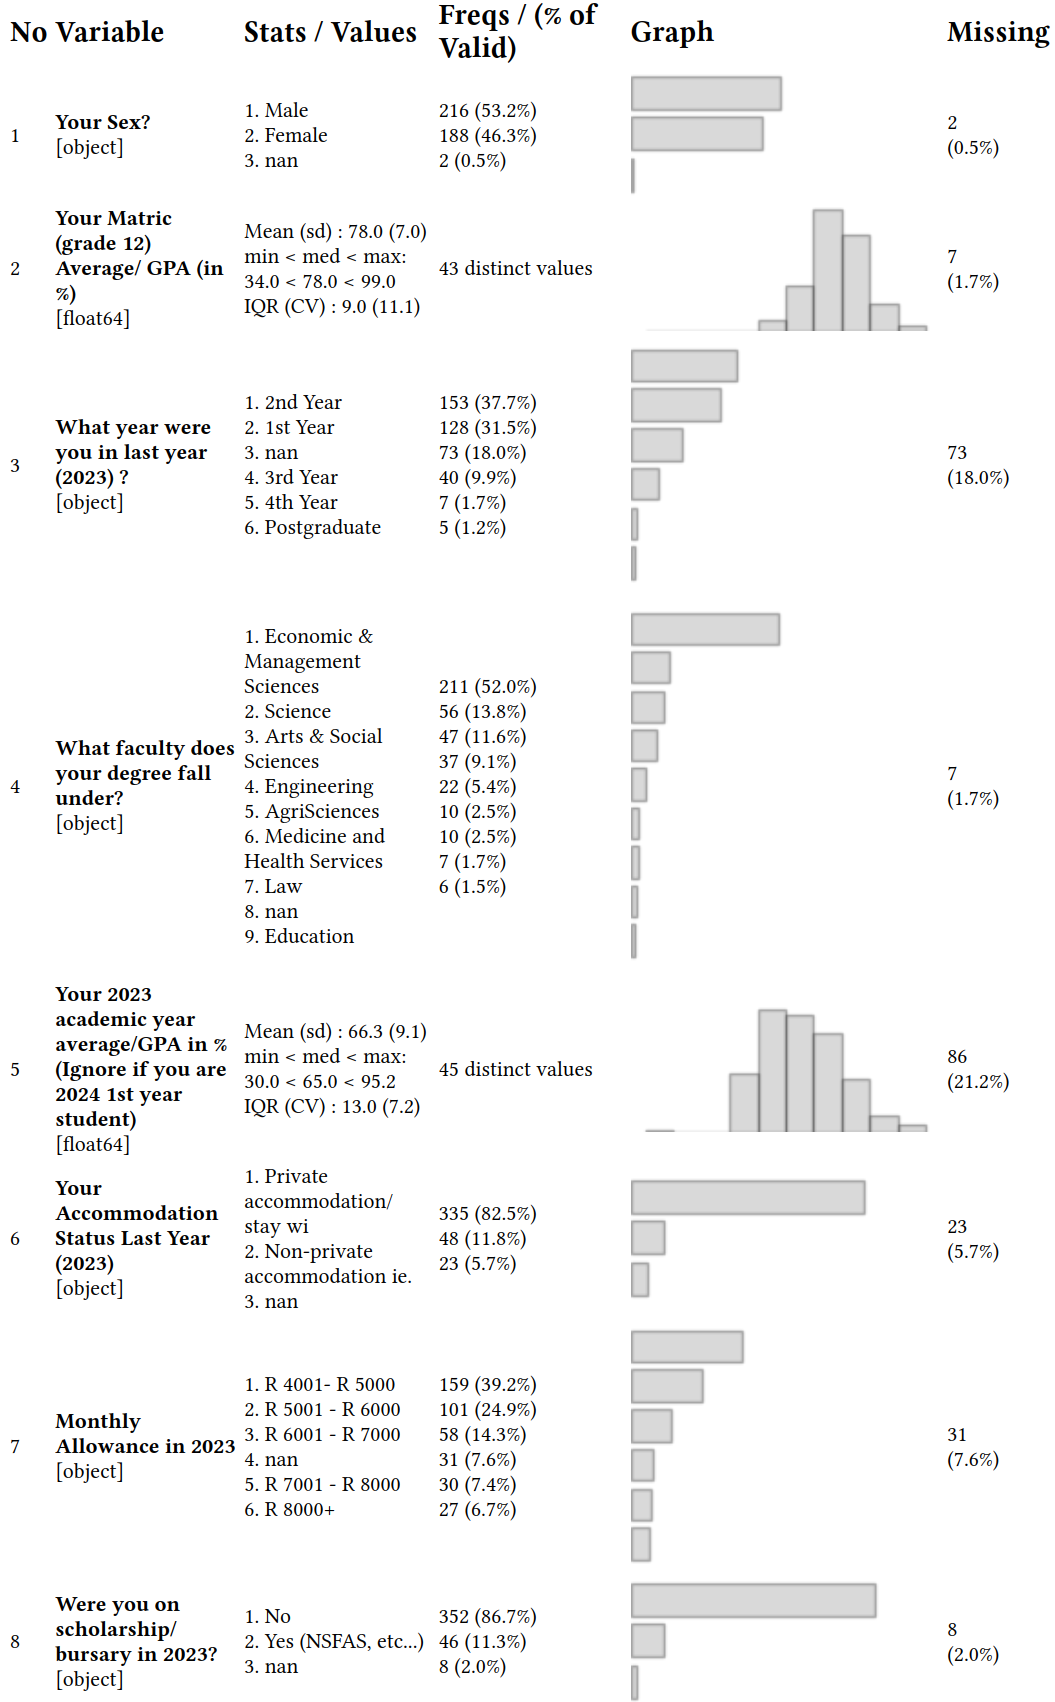
\includegraphics[width=0.9\textwidth]{Tabla1.png}
\end{figure}

\begin{figure}[H]
  \centering
  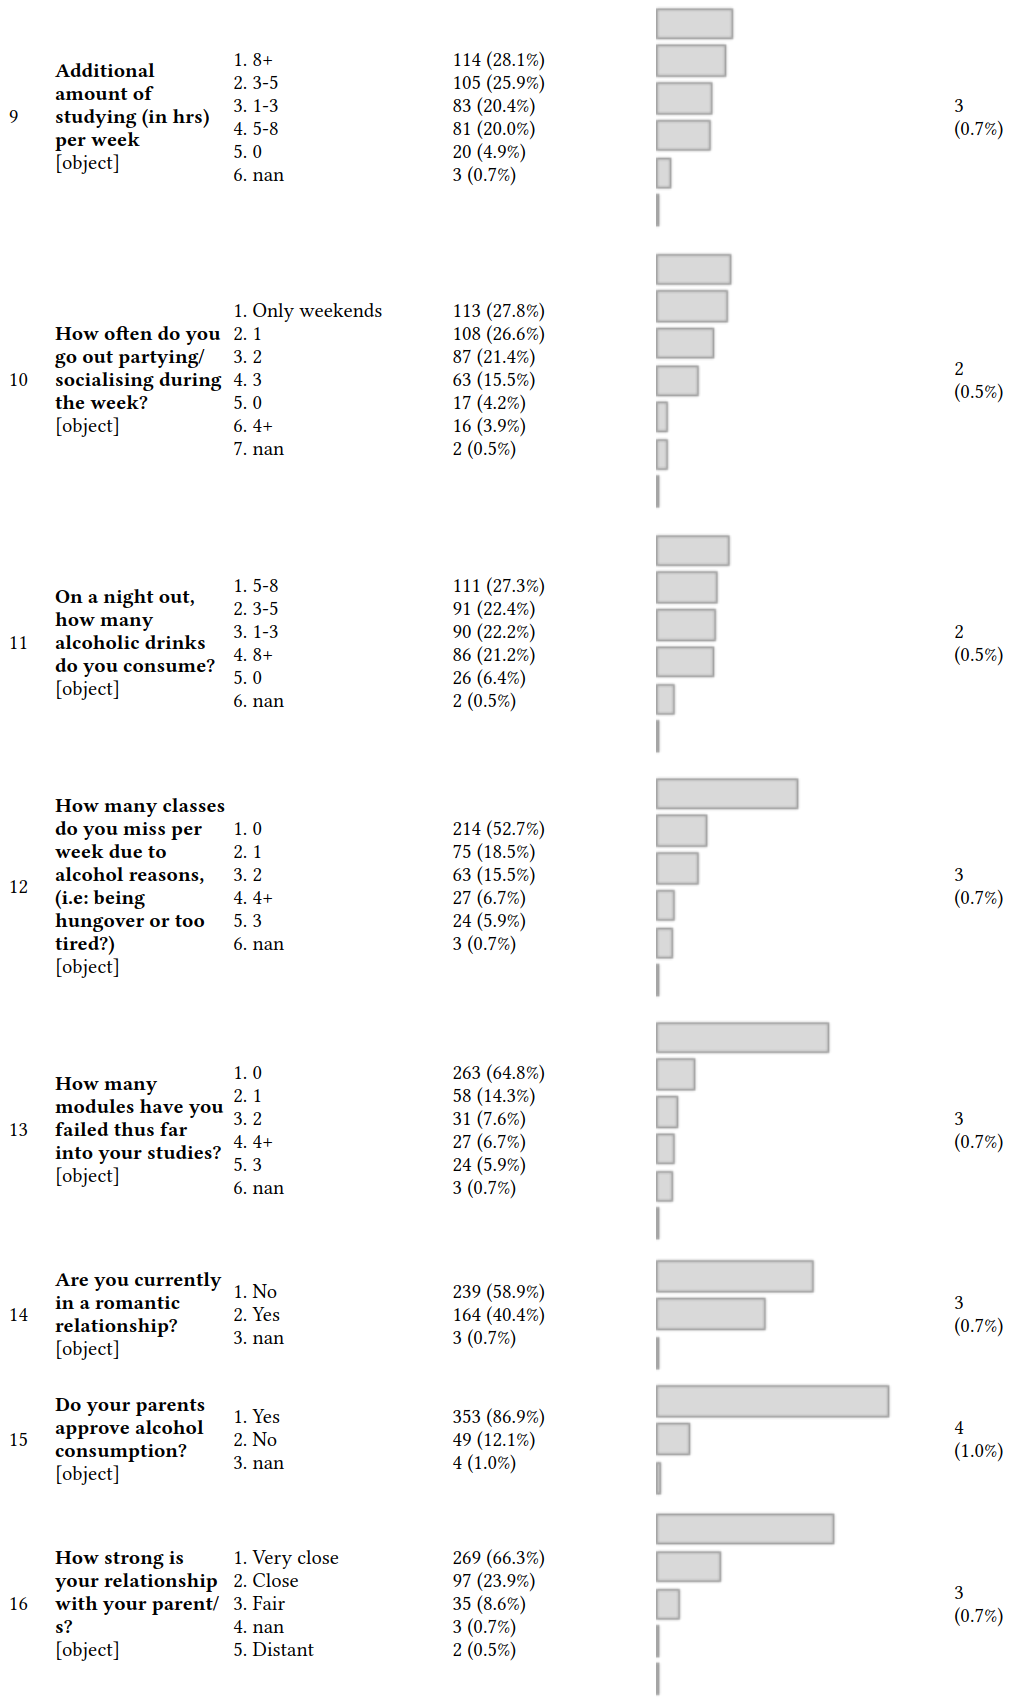
\includegraphics[width=0.9\textwidth]{Tabla2.png}
\end{figure}

\subsection{Preparación de datos}
Antes de la aplicación de un modelo de predicción, es requerido eliminar o imputar datos dentro de ciertos registros. Al realizar un análisis descriptivo de los datos, podemos identificar que los datos en bruto obtenidos desde la encuesta, sobre la pregunta del año académico en el que estuvo cada estudiante el año pasado, existen algunas respuestas que están en blanco, esto quiere decir dichos estudiantes no se encontraban en la Universidad el año anterior. Dado que el modelo va a enfocarse en estudiar exclusivamente a los estudiantes universitarios, se procede a eliminar las entradas incompletas para asegurar el análisis sobre los datos de los estudiantes que estuvieron en la universidad en el año 2023.

La columna numérica "Your 2023 academic year average/GPA in \% (Ignore if you are 2024 1st year student)" será utilizada como nuestra variable objetivo para la clasificación. Se excluirá la columna "Timestamp" del análisis, ya que representa la fecha y hora en la que se realizó la encuesta, y por lo tanto, no será considerada para la creación del modelo de clasificación. Procederemos a separar las columnas en categorías: aquellas que son categóricas y aquellas que son numéricas. La imputación de datos faltantes se llevará a cabo utilizando dos estrategias: para los datos numéricos se empleará la media, y para los datos categóricos se utilizará la moda. Además, se crearán grupos para facilitar la visualización y el análisis de las variables categóricas.

\subsection{Análisis Gráfico.}

\begin{figure}[H]
  \centering
  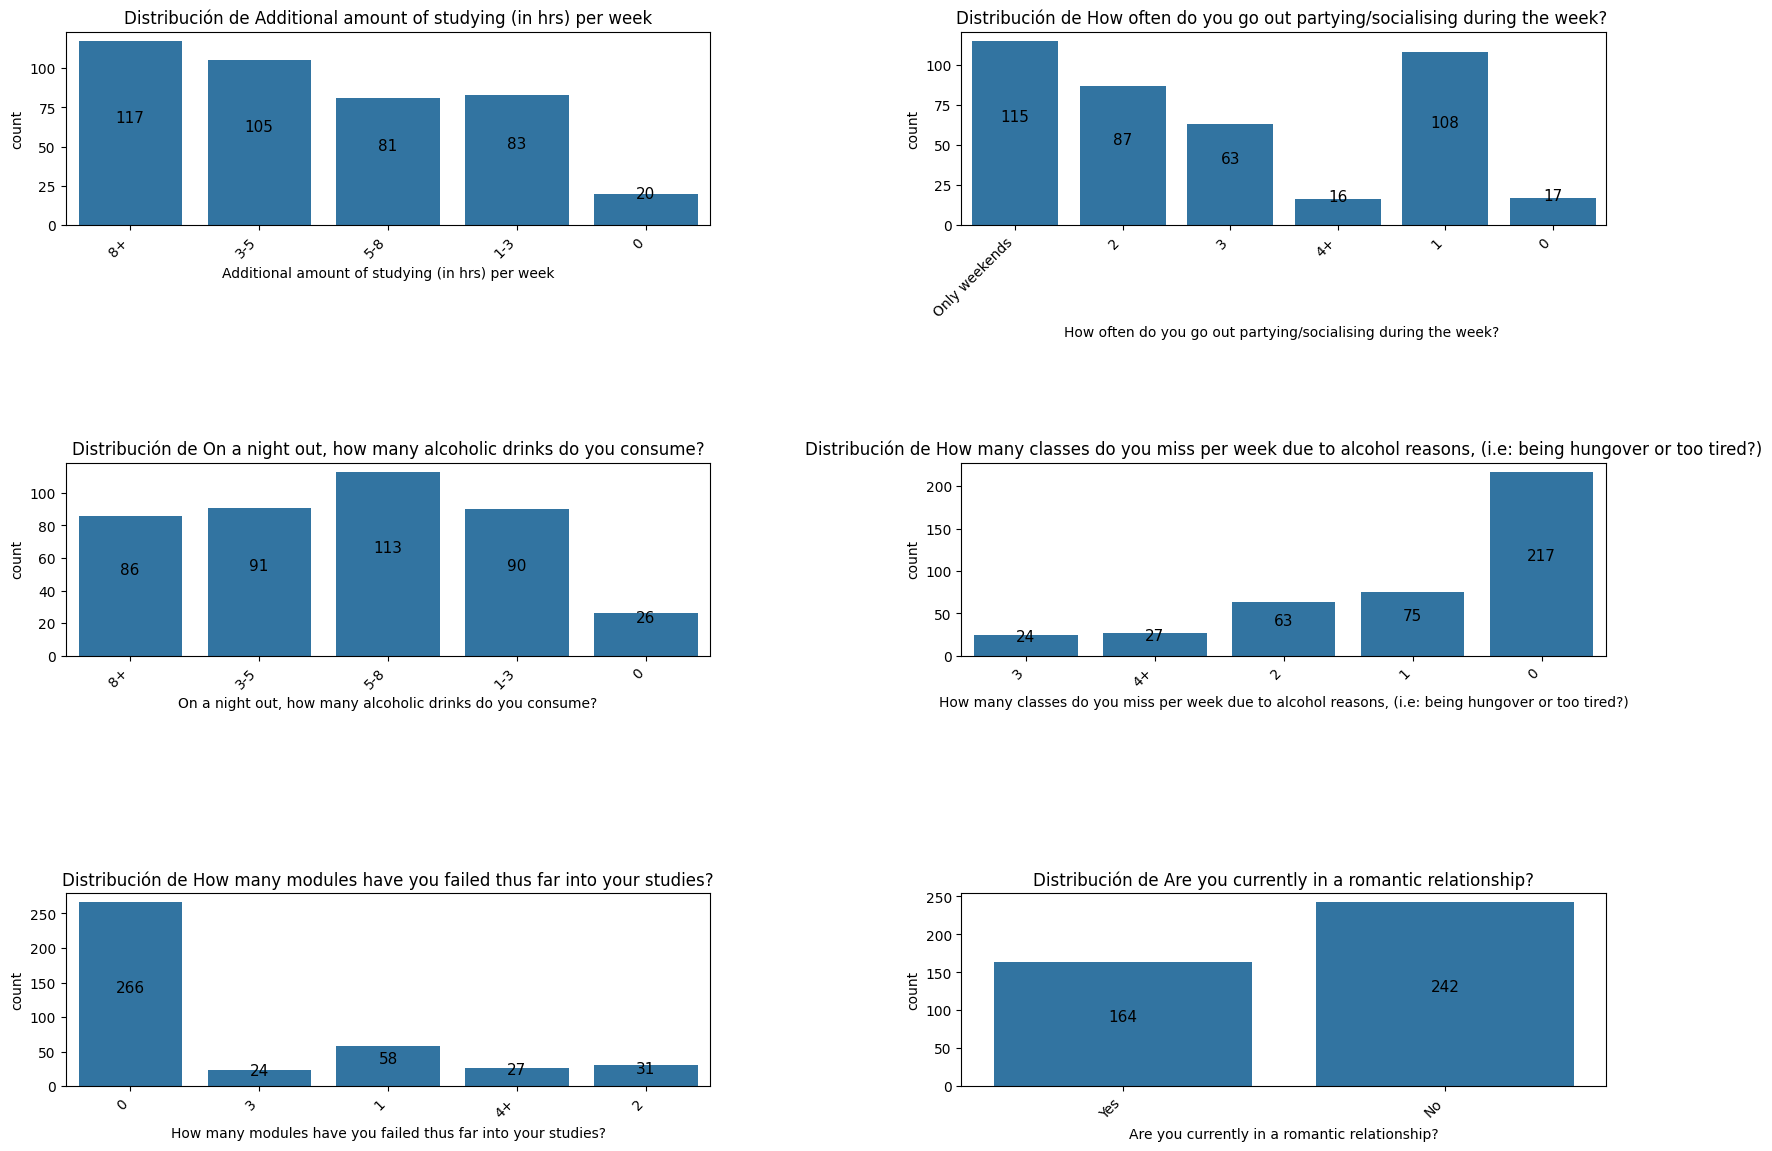
\includegraphics[width=0.9\textwidth]{output1.png}
\end{figure}

A partir de las gráficas anteriores, se pueden destacar los siguientes puntos: La mayoría de los encuestados es de género masculino. En 2023, la mayoría de los encuestados estaban en el primer y segundo año académico. La mayor parte de los encuestados pertenece a la Facultad de Ciencias Económicas y de Gestión. Además, la mayoría de los encuestados viven con familiares. En cuanto al dinero destinado mensualmente, la mayoría de los encuestados recibe entre 4001 y 5001 rands, lo que, al tipo de cambio actual, equivale a entre 224.34 y 280.41 dólares. Finalmente, la mayoría de los encuestados no contaba con una beca en 2023.

\begin{figure}[H]
  \centering
  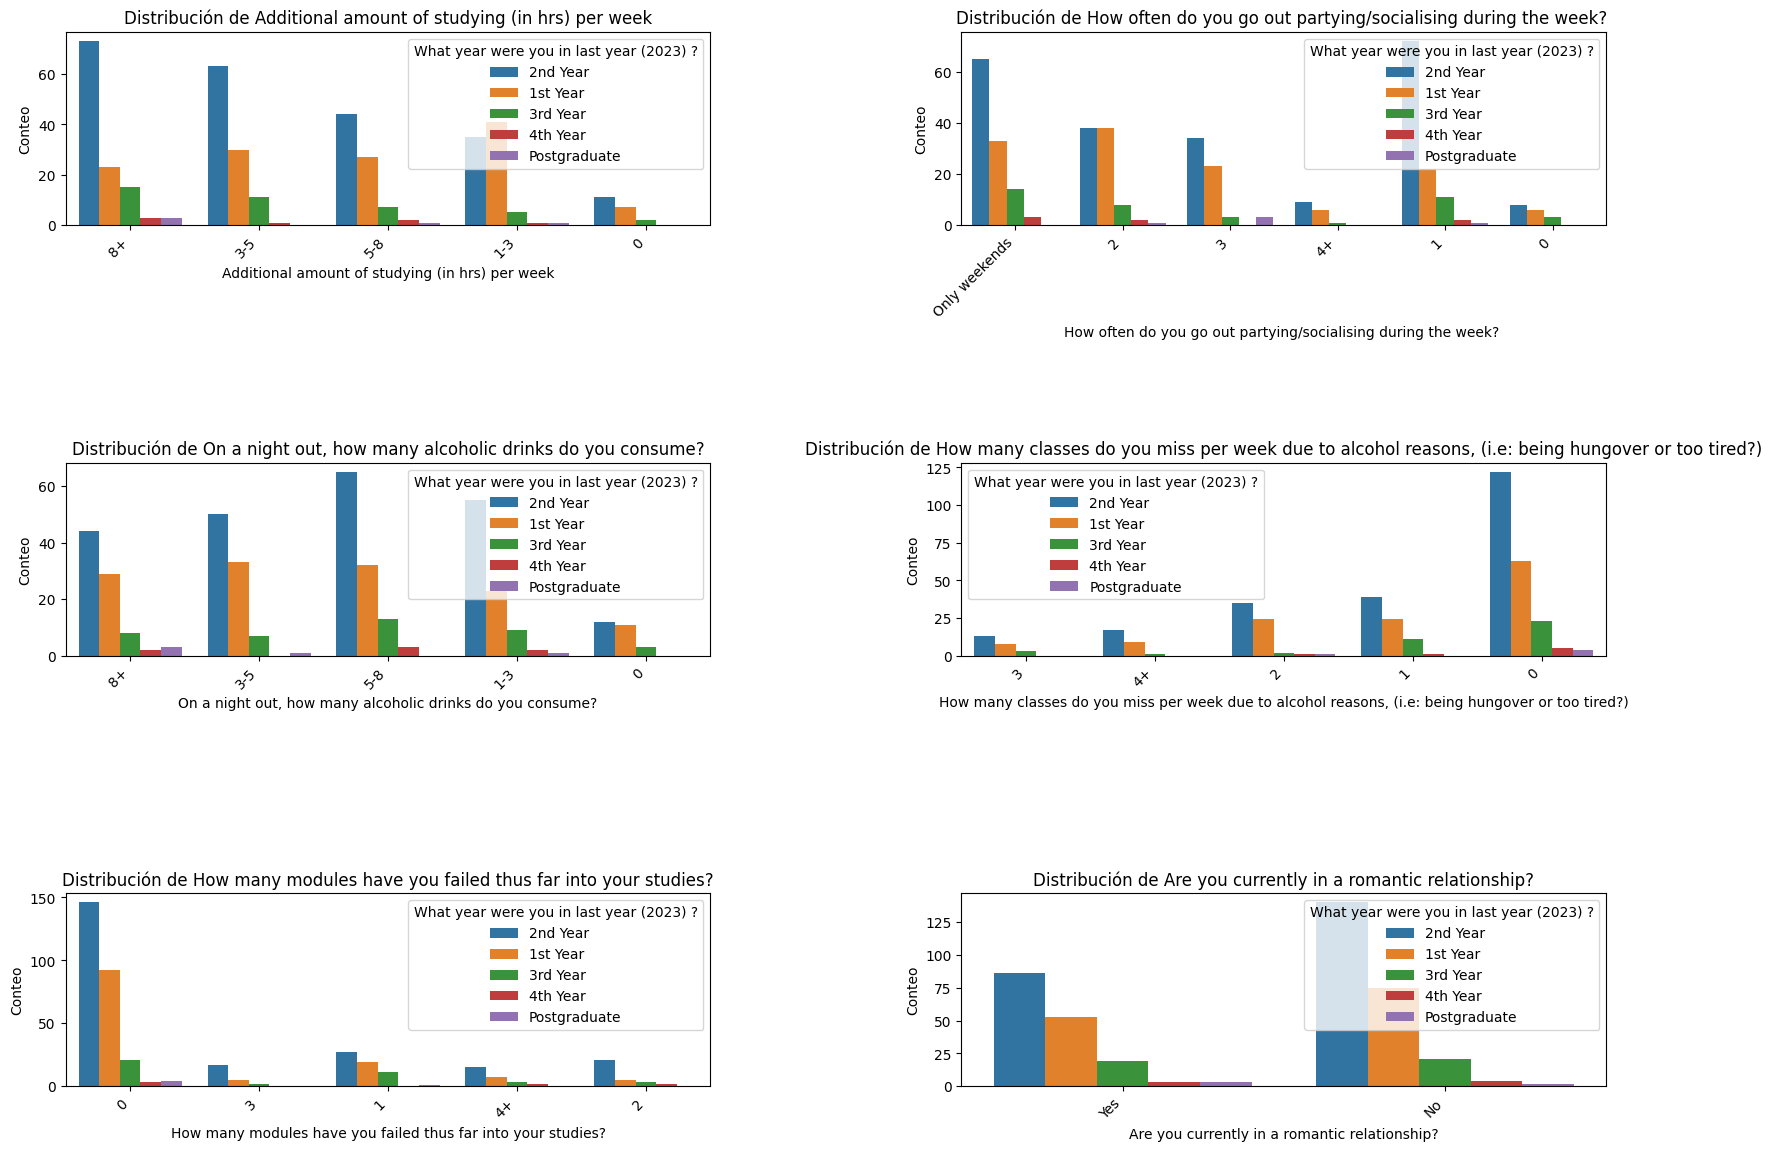
\includegraphics[width=0.9\textwidth]{output3.png}
\end{figure}

Según las gráficas de distribución de cada variable en relación con el año académico que cursaban los estudiantes en 2023, es evidente que la población encuestada se concentra principalmente en estudiantes de primer y segundo año. Esta concentración podría limitar la capacidad para clasificar adecuadamente nuevas entradas, ya que la muestra puede no ser representativa de estudiantes en otros años académicos.

\begin{figure}[H]
  \centering
  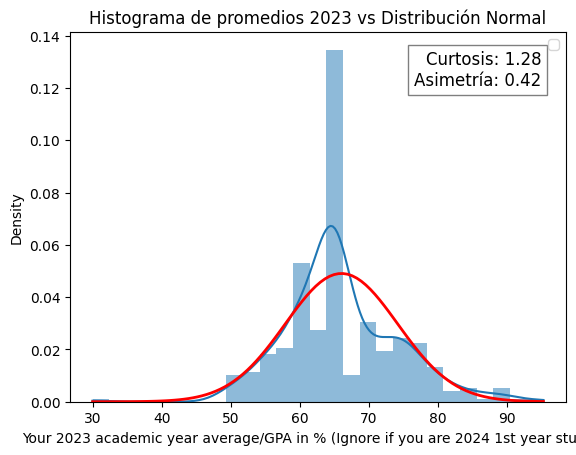
\includegraphics[width=0.75\textwidth]{output4.png}
\end{figure}

Al analizar la normalidad de la variable objetivo relacionada con el rendimiento académico, se observa que una curtosis de 1.28 sugiere colas más ligeras y una menor concentración en el centro en comparación con una distribución normal. Esto indica menos valores extremos y una mayor dispersión alrededor de la media. Asimismo, una asimetría de 0.42 indica una ligera inclinación hacia la derecha, lo que refleja la presencia de un número reducido de observaciones con valores superiores al promedio que alargan la distribución en esa dirección.

\subsection{Aplicación de modelos.}

\begin{figure}[H]
  \centering
  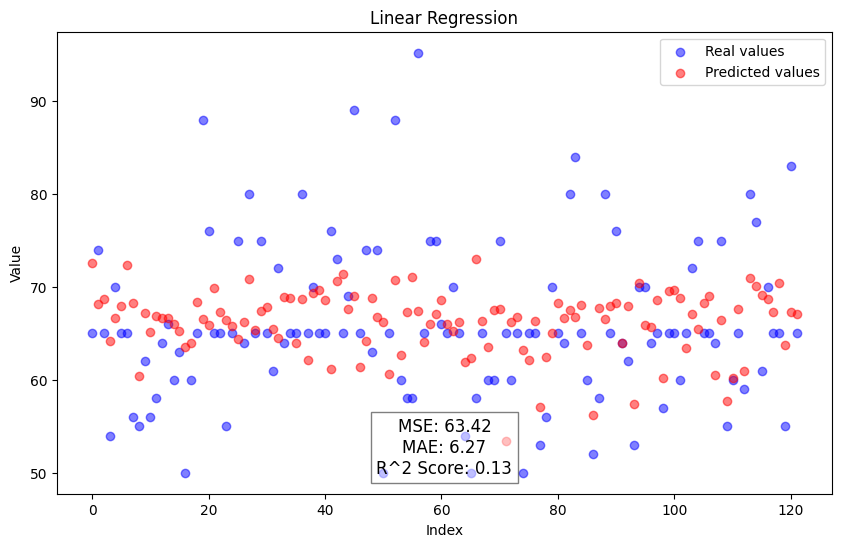
\includegraphics[width=0.75\textwidth]{output5.png}
\end{figure}

El gráfico muestra que el modelo de regresión lineal tiene un bajo rendimiento, como lo indican un MSE de 63.42, un MAE de 6.27 y un R² de 0.13, lo que sugiere que solo el 13\% de la variabilidad de los datos es explicada por el modelo, reflejando una débil capacidad predictiva. Visualmente, los valores predichos (en rojo) no se alinean bien con los valores reales (en azul), lo que confirma estas métricas. Este resultado sugiere que el modelo no es adecuado para estos datos, posiblemente debido a la falta de una relación lineal significativa, la omisión de variables importantes o la necesidad de un modelo más complejo. Se aplicaron técnicas más avanzadas como los modelos de árboles de decisión, o técnicas de machine learning como Random Forest, pero sin embargo se obtuvieron iguales o peores resultados a los obtenidos con Regresión Lineal.

\section{Resultados y Discusión}
El MSE obtenido es de 64.42, lo que indica que, en promedio, el modelo tiene un error cuadrático de aproximadamente 64.42 unidades. En el contexto de rendimiento académico, esto sugiere que las predicciones del modelo pueden tener un margen de error considerable, lo cual puede afectar la precisión general del modelo. \\
\\
El coeficiente R² es de 0.13, significa que el modelo explica una pequeña fracción de la variabilidad en el rendimiento académico, lo que sugiere que hay otros factores no incluidos en el modelo que están influyendo en las calificaciones aparte de los problemas relacionados con el alcohol. \\
\\
Los resultados obtenidos reflejan que el modelo de regresión lineal actual tiene limitaciones significativas. El bajo valor de R² sugiere que el modelo no captura adecuadamente la complejidad del rendimiento académico de los estudiantes. Esto puede ser indicativo de varios problemas, como la falta de variables importantes en el modelo, o la influencia de factores externos no considerados. \\
\\
El MSE relativamente alto también indica que las predicciones del modelo tienen un margen de error considerable. Esto refuerza la necesidad de mejorar el pre-procesamiento de datos y considerar la inclusión de variables adicionales o la utilización de técnicas de modelado más avanzadas. Además, el análisis de la relación entre el consumo de alcohol y el rendimiento académico sugiere que puede haber una interacción significativa que no está siendo capturada adecuadamente por el modelo actual.


\section{Conclusiones}
El estudio ha demostrado que un preprocesamiento adecuado de los datos es esencial para lograr una predicción precisa del rendimiento académico. La normalización y la codificación efectiva de las variables contribuyen a mejorar el rendimiento del modelo de regresión lineal. Además, se observó que ciertas variables relacionadas con el consumo de alcohol tienen una influencia significativa en el rendimiento académico de los estudiantes. Esto sugiere que el análisis de factores asociados con el consumo de alcohol es crucial para comprender su impacto en el rendimiento académico. Aunque el análisis conjunto de todas las variables ofrece una perspectiva general, resulta más efectivo centrarse en aquellas variables que muestran una alta correlación con el rendimiento académico. De esta manera, se pueden desarrollar estrategias más precisas y dirigidas para abordar el impacto del consumo de alcohol y mejorar los resultados académicos de los estudiantes.

\section{Recomendaciones}

La encuesta plantea preguntas valiosas para evaluar el impacto del consumo de alcohol en el rendimiento académico. Es fundamental que la muestra poblacional sea representativa para obtener una visión general y precisa del estudio. En este caso, se observa que la mayoría de los encuestados son estudiantes de primer año, donde el consumo de alcohol puede no ser prioritario frente a sus estudios, aunque esto podría variar según las diferencias culturales y personales. \\
\\
Recomendamos mejorar la selección de la muestra poblacional, incluyendo más encuestados de todos los años académicos disponibles, lo que aportaría mayor variabilidad a las respuestas. Además, sugerimos reducir el número de categorías en las variables, limitándolas a un máximo de tres opciones. Actualmente, algunas variables cuentan con hasta cinco categorías, lo que puede introducir sesgos en los datos. Agrupar mejor las respuestas potenciales podría aumentar la claridad y precisión de los resultados.

\nocite{*}

\bibliographystyle{plain} % Estilo de bibliografía (puede ser otro como alpha, abbrv, etc.)
\bibliography{referencias} % Sin la extensión .bib

\end{document}